\documentclass[pra, onecolumn, notitlepage, floats, 11pt]{revtex4-1}

\usepackage[T1]{fontenc}
\usepackage{graphicx}
\usepackage{color}
\usepackage{latexsym,amsmath}
\usepackage{comment}
\usepackage{tabularx}
\usepackage{siunitx}
\usepackage{multirow}
\usepackage{mathtools}
\usepackage{tikz, fp}
\usepackage{wrapfig}
\usepackage{amsfonts}
\usepackage[pdftex,colorlinks=true, pdfstartview=FitV, linkcolor=linkcolor, citecolor=linkcolor, urlcolor=linkcolor, hyperindex=true,hyperfigures=true]{hyperref} %hyperlink%
\usepackage{fancyhdr}
\usepackage{inconsolata}
\usepackage{listings}
\usepackage{physics}
\usepackage{datetime}
\usepackage[caption=false]{subfig}
\usepackage{titlesec}

\renewcommand{\figurename}{Figure}
\renewcommand{\tablename}{Table}
\renewcommand{\thetable}{\arabic{table}}

\definecolor{airforceblue}{rgb}{0.36, 0.54, 0.66}  %#5D8AA8
\definecolor{cobalt}{rgb}{0.0, 0.28, 0.67}         %#0047AB
\definecolor{coolblack}{rgb}{0.0, 0.18, 0.39}      %#002E63
\definecolor{dartmouthgreen}{rgb}{0.05, 0.5, 0.06} %#00693E
\definecolor{lava}{rgb}{0.81, 0.06, 0.13}          %#CF1020
% move section headings to left
% \sffamily
% \scshape
%\titleformat{\section}{\raggedright\sffamily\bfseries\fontsize{13pt}{13}\selectfont}{\arabic{section}}{1em}{\MakeUppercase}
\titleformat{\section}{\raggedright\bfseries\scshape\fontsize{13pt}{13}\selectfont}{\color{cobalt}\arabic{section}}{1em}{\color{cobalt}}
\titleformat{\subsection}{\raggedright\bfseries\scshape\fontsize{12pt}{12}\selectfont}{{\color{cobalt}\arabic{section}.\arabic{subsection}}}{1em}{\color{cobalt}}
\renewcommand{\thesection}{\arabic{section}}
\renewcommand{\thesubsection}{\arabic{subsection}}
\renewcommand{\thesubsubsection}{\arabic{subsubsection}}
\makeatletter
\renewcommand{\p@subsection}{\thesection.}
\renewcommand{\p@subsubsection}{\thesection.\thesubsection.}
\makeatother


\linespread{0.956}

\DeclarePairedDelimiter\ceil{\lceil}{\rceil}
\DeclarePairedDelimiter\floor{\lfloor}{\rfloor}

\definecolor{linkcolor}{rgb}{0,0,0.65}
\definecolor{shadecolor}{rgb}{0.95, 0.95, 0.95}
\definecolor{mygreen}{rgb}{0,0.6,0}
\definecolor{mygray}{rgb}{0.5,0.5,0.5}
\definecolor{mymauve}{rgb}{0.58,0,0.82}
\lstdefinestyle{fortran}
{
    backgroundcolor=\color{shadecolor},       % background color
    basicstyle=\ttfamily\footnotesize,        % the size of the fonts that are used for the code
    breakatwhitespace=false,                  % sets if automatic breaks should only happen at whitespace
    breaklines=false,                         % sets automatic line breaking
    captionpos=b,                             % sets the caption-position to bottom
    commentstyle=\color{mygreen},             % comment style
    extendedchars=true,                       % lets you use non-ASCII characters; for 8-bits encodings only, does not work with UTF-8
    keepspaces=true,                          % keeps spaces in text, useful for keeping indentation of code (possibly needs columns=flexible)
    keywordstyle=\bfseries\color{blue},       % keyword style
    language=[95]Fortran,                     % the language of the code
    numbers=left,                             % where to put the line-numbers; possible values are (none, left, right)
    numbersep=5pt,                            % how far the line-numbers are from the code
    numberstyle=\tiny\color{mygray},          % the style that is used for the line-numbers
    rulecolor=\color{black},                  % if not set, the frame-color may be changed on line-breaks within not-black text (e.g. comments (green here))
    showspaces=false,                         % show spaces everywhere adding particular underscores; it overrides 'showstringspaces'
    showstringspaces=false,                   % underline spaces within strings only
    showtabs=false,                           % show tabs within strings adding particular underscores
    stepnumber=1,                             % the step between two line-numbers. If it's 1, each line will be numbered
    stringstyle=\color{mymauve},              % string literal style
    tabsize=4,                                % sets default tabsize to 4 spaces
    title=\lstname                            % show the filename of files
}

\lstdefinestyle{python}
{
    backgroundcolor=\color{shadecolor},       % background color
    basicstyle=\ttfamily\footnotesize,        % the size of the fonts that are used for the code
    breakatwhitespace=false,                  % sets if automatic breaks should only happen at whitespace
    breaklines=false,                         % sets automatic line breaking
    captionpos=b,                             % sets the caption-position to bottom
    commentstyle=\color{mygreen},             % comment style
    extendedchars=true,                       % lets you use non-ASCII characters; for 8-bits encodings only, does not work with UTF-8
    keepspaces=true,                          % keeps spaces in text, useful for keeping indentation of code (possibly needs columns=flexible)
    keywordstyle=\bfseries\color{blue},       % keyword style
    language=Python,                          % the language of the code
    numbers=left,                             % where to put the line-numbers; possible values are (none, left, right)
    numbersep=5pt,                            % how far the line-numbers are from the code
    numberstyle=\tiny\color{mygray},          % the style that is used for the line-numbers
    rulecolor=\color{black},                  % if not set, the frame-color may be changed on line-breaks within not-black text (e.g. comments (green here))
    showspaces=false,                         % show spaces everywhere adding particular underscores; it overrides 'showstringspaces'
    showstringspaces=false,                   % underline spaces within strings only
    showtabs=false,                           % show tabs within strings adding particular underscores
    stepnumber=1,                             % the step between two line-numbers. If it's 1, each line will be numbered
    stringstyle=\color{mymauve},              % string literal style
    tabsize=4,                                % sets default tabsize to 4 spaces
    title=\lstname                            % show the filename of files
}


\pagestyle{fancy}
\fancyhf{}
\fancyhead[L]{Rocco Ardino (Mat. 1231629)}
\fancyhead[R]{\bf\thepage}
\fancyfoot[L]{\textsc{report}: Week 5}
\fancyfoot[R]{\today}
\renewcommand{\headrulewidth}{0.1pt}
\renewcommand{\footrulewidth}{0.1pt}

\newcommand{\codebold}[2][cobalt]{\texttt{\bfseries {\color{#1}#2}}}
\newcommand{\code}[2][black]{\color{#1}\texttt{#2}}
\newcommand{\codefunctionbold}[2]{\texttt{\bfseries {\color{cobalt}#1}({\color{lava}#2})}}
\newcommand{\codefunction}[2]{\texttt{#1(#2})}










\begin{document}

\title{Quantum Information and Computing 2020/21\\Week 5 report}

\author{Rocco Ardino}

\date{\today}





\begin{abstract}
    In this work we deal with eigenvalue problems using Lapack library functions. In particular, we focus on large enough random hermitian matrices and we analyze the normalized spacings between eigenvalues. Then, after a proper handling, we compare the extracted data with a theoretical distribution and find out if the expectation is met.
\end{abstract}

\maketitle




\section{Theory}
Given a random hermitian matrix \( A \) of dimensions \( n \times n \), it follows from the spectral theorem that \( A \) can be diagonalized by a unitary matrix, and that the resulting diagonal matrix has only real entries. This implies that all eigenvalues of a \( A \) are real, and that \( A \) has \( n \) linearly independent eigenvectors.

Denoting with \( \lambda_{i} \) the eigenvalues of \( A \), with \( i = 1, \dots, n \) and \( \lambda_{1} \le \lambda_{2} \le \dots \le \lambda_{n} \), the normalized spacings between them can be computed as:
\begin{equation}
    s_{i}
    =
    \frac{\lambda_{i+1} - \lambda_{i}}{\expval{\Delta \lambda}}
    \quad ,
    \label{eq:05_T_1}
\end{equation}
where \( \expval{\Delta \lambda} \) is the average of \( \Delta \lambda_{i} = \lambda_{i+1} - \lambda_{i} \). In particular, the \( s_{i} \) can be either computed:
\begin{itemize}
    \item globally, by considering as normalization the average of all spacings;
    \item locally, by considering as normalization for the \( i^{\text{th}} \) spacing the averange of only the \( s_{j} \) such that \( j = i-\ell, \dots, i+\ell \), with \( \ell \) a parameter called level.
\end{itemize}

We expect that the distribution of the normalized spacings will be the so-called Wigner surmise, which reads:
\begin{equation}
    P(s)
    =
    \frac{32}{\pi^2} s^2 e^{-\frac{4}{\pi} s^2}
    \quad .
    \label{eq:05_T_2}
\end{equation}
A good strategy is to sample a set of normalized spacings from multiple matrices like \( A \), bin the sampled data and normalize them, then fit with the following function:
\begin{equation}
    P(s)
    =
    a s^{\alpha} e^{-b s^{\beta}}
    \quad .
    \label{eq:05_T_3}
\end{equation}

Lastly, an interesting quantity can be computed from the normalized spacings. We start from the following quatities
\begin{equation}
    r_{i}
    =
    \frac{\min\qty{\Delta\lambda_{i}, \Delta\lambda_{i+1}}}{\max\qty{\Delta\lambda_{i}, \Delta\lambda_{i+1}}}
    \quad .
    \label{eq:05_T_4}
\end{equation}
From this set, computed for \( i = 1, \dots, n-2 \), we can get the average \( \expval{r} \).





\section{Code Development}
For this work, the new module \codebold{hmat} is implemented, containing several functions and subroutines for multiple purposes:
\begin{itemize}
    \item \codebold{random\_normal}, for generating random normal distributed numbers;
    \item \codefunctionbold{hmat\_init}{dim}, for creating a generic hermitian matrix of dimensions \( n \times n \) with random normal entries;
    \item \codefunctionbold{hmat\_diag\_init}{dim}, for creating a diagonal hermitian matrix of dimensions \( n \times n \) with random normal entries;
    \item \codefunctionbold{hmat\_eigs}{a}, which returns the eigenvalues of the hermitian matrix \code{a};
    \item \codefunctionbold{hmat\_s}{eigs}, which returns the globally normalized spacings \( s_{i} \), given the eigenvalues \code{eigs};
    \item \codefunctionbold{hmat\_s\_loc}{eigs, level}, which works like \code{hmat\_s}, but it reurns the locally normalized spacings, computed with the \code{level} parameter;
    \item \codefunctionbold{hmat\_r\_avg}{eigs, filename, unit}, for calculating the quantity \( \expval{r} \) and storing it in a file;
    \item \codefunctionbold{hist2pdf}{data, min, max, nbins, filename, unit}, for binning the given \code{data} in a certain number of bins in an interval \( [x_{\mathrm{min}}, x_{\mathrm{max}}] \), and for normalizing to a PDF the result, storing the normalized bin centers and heights in a file.
\end{itemize}

In particular, we explain the core functionalities in the following subsections.



\subsection{Eigenvalues and spacings computation}
For the calculations of the eigenvalues of a complex hermitian matrix, the Lapack function \codebold[black]{zheev} is employed. Therefore, the function \codebold[black]{hmat\_eigs} is built as a wrapper of the Lapack function, as it is showed in Listing \ref{lst:05_C_SS_1_1}.

\medskip
\begin{lstlisting}[
    style=fortran,
    frame=single,
    label={lst:05_C_SS_1_1},
    caption={Implementation of the wrapper of \code{zheev}.}
]
function hmat_eigs(a) result(eigs)
    complex(8), dimension(:,:) :: a

    real(8), dimension(lbound(a,dim=1):ubound(a,dim=1)) :: eigs
    complex(8), dimension(:), allocatable :: work(:)
    real(8),    dimension(:), allocatable :: rwork(:)
    integer(4) :: N
    integer(4) :: lwork, info

    N     = size(a, 1)
    lwork = max(1,2*N-1)

    allocate(work(lwork))
    allocate(rwork(max(1, 3*N-2)))
    call zheev('N', 'U', N, a, N, eigs, work, lwork, rwork, info)
    deallocate(work)
    deallocate(rwork)
end function hmat_eigs
\end{lstlisting}

For the calculation of the spacings, \code{hmat\_eigs} is called in both global and local implementations to get firstly the eigenvalues. Then, some other algebraic operations are performed in order to get the spacings, as it can be seen in Listing \ref{lst:05_C_SS_1_2} and \ref{lst:05_C_SS_1_3} respectively for the global and local version.

\medskip
\begin{lstlisting}[
    style=fortran,
    frame=single,
    label={lst:05_C_SS_1_2},
    caption={Function for the calculation of the globally normalized spacings.}
]
function hmat_s(eigs) result(s)
    real(8), dimension(:)  :: eigs

    real(8), dimension(lbound(eigs,dim=1):(ubound(eigs,dim=1)-1)) :: s
    real(8) :: s_m
    integer(4) :: ii

    do ii=1,size(eigs,1)-1
        s(ii) = eigs(ii+1) - eigs(ii)
    end do

    s_m = (eigs(size(eigs,1)) - eigs(1)) / size(s,1)

    do ii=1,size(s,1)
        s(ii) = s(ii) / s_m
    end do
end function hmat_s
\end{lstlisting}

\begin{lstlisting}[
    style=fortran,
    frame=single,
    label={lst:05_C_SS_1_3},
    caption={Function for the calculation of the locally normalized spacings.}
]
function hmat_s_loc(eigs, level) result(s)
    real(8), dimension(:)  :: eigs

    integer(4) :: level
    real(8), dimension(lbound(eigs,dim=1):(ubound(eigs,dim=1)-1)) :: s
    integer(4) :: ii, ll, uu


    do ii=1,size(s,1)
        ll = MAX(1, ii-level)
        uu = MIN(size(s,1), ii+level)
        s(ii) = (eigs(ii+1) - eigs(ii)) / ((eigs(uu) - eigs(ll)) / (uu-ll+1))
    end do
end function hmat_s_loc
\end{lstlisting}



\subsection{\( P(s) \) PDF construction}
After having computed the normalized spacings, the subroutine \codebold[black]{hist2pdf} takes the list of spacings and starts to fill a histogram with a given number of bins in a defined interval. Then, it normalizes every bin height with the total number of entries and the bin width. It finally creates a file and fills it with the bin centers and normalized heights. The whole simplified operation is showed in Listing \ref{lst:05_C_SS_2_1}.

\medskip
\begin{lstlisting}[
    style=fortran,
    frame=single,
    label={lst:05_C_SS_2_1},
    caption={Subroutine for the creation of a PDF from histogram data.}
]
subroutine hist2pdf(data, min, max, nbins, filename, unit)
    ! input arguments
    real(8), dimension(:) :: data
    real(8) :: min, max
    integer(4) :: nbins
    character(*) :: filename
    integer(4) :: unit

    real(8), dimension(nbins) :: binc, binh
    real(8) :: binw
    integer(4) :: ii, jj
    logical :: bin_inf, bin_sup, x_inf, x_sup

    ! set to zero bin centers and heights
    binc = 0
    binh = 0

    ! define bin centers
    binw = (max - min) / nbins
    do ii=1,size(binc)
        binc(ii) = min + (ii-0.5)*binw
    end do

    ! fill bins (~define bin heights)
    do ii=1,size(data,1)
        do jj=1,nbins
            bin_inf = data(ii) > (min + (jj-1)*binw)
            bin_sup = data(ii) < (min +  jj   *binw)
            x_inf   = data(ii) > min
            x_sup   = data(ii) < max
            if (bin_inf .AND. bin_sup .AND. x_inf .AND. x_sup) then
                binh(jj) = binh(jj) + 1
            end if
        end do
    end do

    ! normalize bin heights to get a pdf
    do ii=1,size(binh,1)
        binh(ii) = binh(ii) / (size(data,1)*binw)
    end do

    ! write results on file to use for plotting
    open(unit, file=filename, status='replace')
    do ii=1,size(binc,1)
        write(unit,'(g0ag0)') binc(ii), char(9), binh(ii)
    end do
    close(unit)
end subroutine hist2pdf
\end{lstlisting}



\subsection{Test program and automatization}
Lastly, all the functions described before are employed in a test program on multiple samples, i.e. hermitian matrices, for both glabal and local case and for both random hermitian and random diagonal matrices. The program takes multiple command-line input arguments, listed in Table \ref{tab:05_C_SS_3_1}.

\begin{table}[!h]
    \begin{tabular}{ccc}
        \toprule
        Arg name    &   Arg number  &   Arg meaning \\
        \colrule
        \code{h\_type}  &   1   &   Type of hermitian matrix (herm=generic, diag=diagonal)  \\
        \code{samples}  &   2   &   Number of matrices from which spacings are sampled  \\
        \code{N}        &   3   &   Dimension of sampled matrices   \\
        \code{nbins}    &   4   &   Number of bins for the PDF  \\
        \code{xmin}     &   5   &   Lower bound for the histogram   \\
        \code{xmax}     &   6   &   Upper bound for the histogram   \\
        \code{local}    &   7   &   Enable local average (1) or disable (otherwise) \\
        \code{level}    &   8   &   Level parameter if local average is enabled \\
        \botrule
    \end{tabular}
    \caption{Command-line arguments of the test program.}
    \label{tab:05_C_SS_3_1}
\end{table}

In order to compile the program and for an easy debugging, \code{-Wall} and \code{-ffree-line-length-0} flags are added and the Lapack library is linked. Then, a Python script is implemented to call the Fortran executable for all the possible cases, saving every result in a dedicated folder.



\section{Results}
To sample a sufficient amount of data for the fit, the spacings for a \( 2500 \times 2500 \) random hermitian matrix are sampled for 50 times. Moreover, this procedure is done for both diagonal and generic hermitian matrices and for both global and local average implementations. The number of bins chosen is 100 and the range is the interval \( [0,5] \). Lastly, the quantity \( \expval{r} \) is computed in every case. The results are showed in Figures \ref{fig:05_R_1} and \ref{fig:05_R_2}, obtained through a Gnuplot script, and in Table \ref{tab:05_R_1}, where the fit parameters are listed. It is interesting to observe how the fit parameters converge to the expected values from theory when the local average is employed and the level parameter is sufficiently small. This is probably due to the fact that the spacing average becomes more sharp and significant at a local level.

\begin{figure*}[!h]
    \centering
    \subfloat[][{\small Generic hermitian matrices}]{
        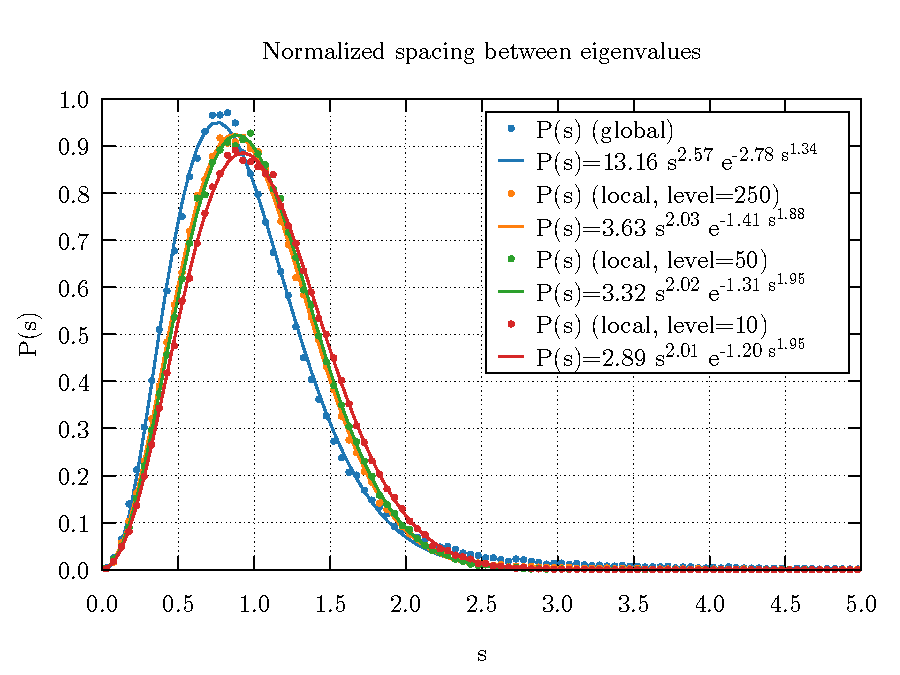
\includegraphics[width=0.48\textwidth]{images/herm_50_samples_2500_N.pdf}
        \label{fig:05_R_1}
    }
    \hfill
    \subfloat[][{\small Diagonal hermitian matrices}]{
        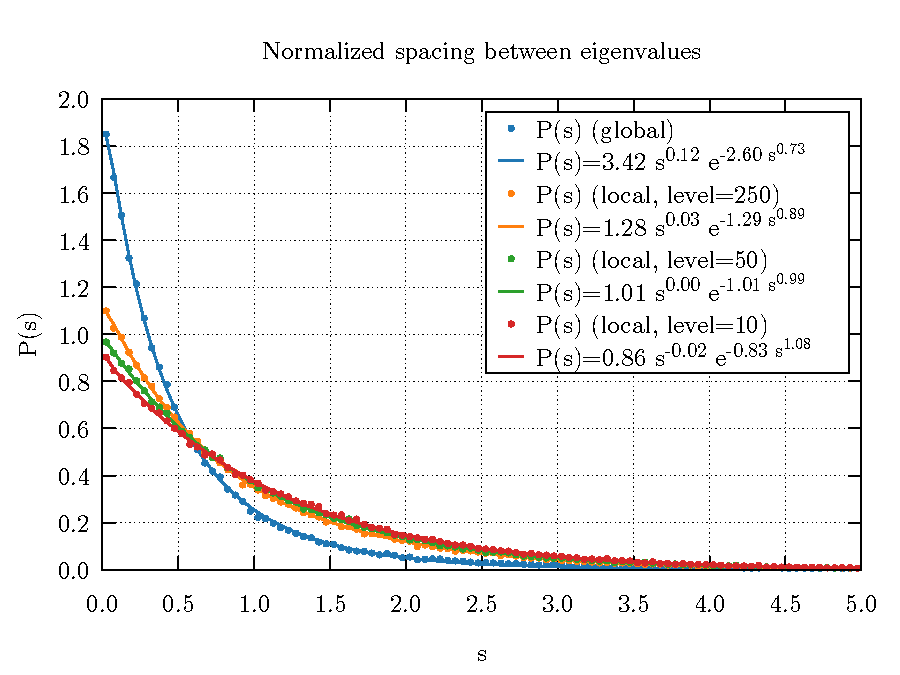
\includegraphics[width=0.48\textwidth]{images/diag_50_samples_2500_N.pdf}
        \label{fig:05_R_2}
    }
    \caption{Results for the normalized spacings between eigenvalues, obtained for both type of matrices and for both local and global implementations of the average spacing. The sampled distributions are showed with points and the corresponding fits with lines of the same color.}
\end{figure*}

\setlength{\tabcolsep}{6pt}
\begin{table}[!h]
    \begin{tabular}{ccccccc}
        \toprule
        H. matrix type  &   Level       &   \( a \) &   \( \alpha \)    &   \( b \) &   \( \beta \) &   \( \expval{r} \)    \\
        \colrule
        generic         &   \( *** \)   &   \( 13    \pm 3    \)    &   \( 2.6   \pm 0.1   \)   &   \( 2.8  \pm 0.2  \) &   \( 1.34 \pm 0.05 \) &   \( 0.5967 \pm 0.0002 \)   \\
        generic         &   \( 250 \)   &   \(  3.6  \pm 0.2  \)    &   \( 2.03  \pm 0.03  \)   &   \( 1.41 \pm 0.04 \) &   \( 1.88 \pm 0.03 \) &   \( 0.6012 \pm 0.0002 \)   \\
        generic         &   \(  50 \)   &   \(  3.3  \pm 0.1  \)    &   \( 2.02  \pm 0.03  \)   &   \( 1.31 \pm 0.04 \) &   \( 1.95 \pm 0.03 \) &   \( 0.6025 \pm 0.0002 \)   \\
        {\bf\color{dartmouthgreen}generic}    &
        {\bf\color{dartmouthgreen}\(\bf 10 \)}   &
        {\bf\color{dartmouthgreen}\(\bf  2.9  \pm 0.1  \)}   &
        {\bf\color{dartmouthgreen}\(\bf 2.01  \pm 0.03 \)}   &
        {\bf\color{dartmouthgreen}\(\bf 1.20 \pm 0.03 \)}    &
        {\bf\color{dartmouthgreen}\(\bf 1.95 \pm 0.03 \)}    &
        {\bf\color{dartmouthgreen}\(\bf 0.5989 \pm 0.0002 \)}\\
        % generic         &   \(  10 \)   &   \(  2.9  \pm 0.1  \)    &   \( 2.01  \pm 0.03  \)   &   \( 1.20 \pm 0.03 \) &   \( 1.95 \pm 0.03 \) &   \( 0.5989 \pm 0.0002 \)   \\
        \colrule
        diagonal        &   \( *** \)   &   \(  3.4  \pm 0.2  \)    &   \( 0.12  \pm 0.01  \)   &   \( 2.60 \pm 0.07 \) &   \( 0.73 \pm 0.02 \) &   \( 0.3859 \pm 0.0002 \)   \\
        diagonal        &   \( 250 \)   &   \(  1.28 \pm 0.03 \)    &   \( 0.029 \pm 0.006 \)   &   \( 1.29 \pm 0.03 \) &   \( 0.89 \pm 0.01 \) &   \( 0.3919 \pm 0.0002 \)   \\
        diagonal        &   \(  50 \)   &   \(  1.01 \pm 0.02 \)    &   \( 0.005 \pm 0.006 \)   &   \( 1.01 \pm 0.02 \) &   \( 0.99 \pm 0.01 \) &   \( 0.3833 \pm 0.0002 \)   \\
        {\bf\color{dartmouthgreen}diagonal}   &
        {\bf\color{dartmouthgreen}\(\bf 10 \)}   &
        {\bf\color{dartmouthgreen}\(\bf  0.86 \pm 0.02 \)}   &
        {\bf\color{dartmouthgreen}\(\bf -0.017 \pm 0.005 \)} &
        {\bf\color{dartmouthgreen}\(\bf 0.83 \pm 0.02 \)}    &
        {\bf\color{dartmouthgreen}\(\bf 1.08 \pm 0.02 \)}    &
        {\bf\color{dartmouthgreen}\(\bf 0.3875 \pm 0.0002 \)}\\
        % diagonal        &   \(  10 \)   &   \(  0.86 \pm 0.02 \)    &   \(-0.017 \pm 0.005 \)   &   \( 0.83 \pm 0.02 \) &   \( 1.08 \pm 0.02 \) &   \( 0.3875 \pm 0.0002 \)   \\
        \botrule
    \end{tabular}
    \caption{Fit results and \( \expval{r} \) for every case analyzed. The best results are highlighted in green.}
    \label{tab:05_R_1}
\end{table}





\section{Self-evaluation}
In this work we managed to work with Lapack library functions and to describe the PDF of the eigenvalue spacings for several cases. The implementation of the code needed for the purpose has led to successful results, in agreement with the theory for the local average case and for a sufficiently small value of the level parameter.

\end{document}
